\section{SEP 2007}  

\important{ADD MISSING EXAMPLES AND THEORY}

\subsection{Processes and Threads}

\begin{example2}{Process vs. Thread Differences}
    Explain the difference between processes and threads:
    
    \tcblower
    
    \textbf{Solution:}
    The main difference is that processes have their own memory space, while threads (belonging to the same process) share the process memory space.
    
    \begin{minipage}{0.5\linewidth}
    \textbf{Processes:}
    \begin{itemize}
        \item Independent memory spaces
        \item Higher creation/switching overhead
        \item Better isolation and fault tolerance
        \item Communication via IPC mechanisms
    \end{itemize}
    \end{minipage}%
    \begin{minipage}{0.5\linewidth}    
    \textbf{Threads:}
    \begin{itemize}
        \item Shared memory space within process
        \item Lower creation/switching overhead
        \item Faster communication via shared memory
        \item Risk of interference between threads
    \end{itemize}
    \end{minipage}
\end{example2}

\begin{KR}{Analyzing Process vs. Thread Questions}
    \paragraph{Key comparison points}
    \begin{itemize}
        \item Memory organization: separate vs. shared address space
        \item Creation overhead: high vs. low
        \item Communication methods: IPC vs. shared memory
        \item Isolation level: strong vs. weak
        \item Context switching cost: expensive vs. cheap
    \end{itemize}
    
    \paragraph{Common exam patterns}
    \begin{itemize}
        \item Define fundamental differences
        \item Compare advantages/disadvantages
        \item Explain when to use which approach
        \item Analyze code examples with fork() vs.\ pthread\_create()
    \end{itemize}
\end{KR}

\important{ADD EXERCISE 1D SEP07 USER VS KERNEL-LEVEL-THREADS}

\begin{example2}{Process Creation with fork()}
    Unix systems use fork() for process creation. Describe the system call:
    
    \tcblower
    
    \textbf{fork() characteristics:}
    \begin{itemize}
        \item \textbf{Parameters}: None
        \item \textbf{Return value}: Process ID (PID)
            \begin{itemize}
                \item Parent process receives child's PID
                \item Child process receives 0
                \item Error case returns -1
            \end{itemize}
        \item \textbf{Behavior}: Creates exact copy of calling process
    \end{itemize}
    
\begin{lstlisting}[language=C, style=basesmol]
#include <stdio.h>
#include <unistd.h>

int main() {
    pid_t pid = fork();
    
    if (pid < 0) {
        // Error occurred
        perror("Fork failed");
    } else if (pid == 0) {
        // Child process
        printf("Child process: PID = %d\n", getpid());
    } else {
        // Parent process
        printf("Parent: Child PID = %d\n", pid);
    }
    
    return 0;
}
\end{lstlisting}
\end{example2}

\begin{KR}{Process Creation Analysis}
    \paragraph{fork() behavior pattern}
    \begin{itemize}
        \item One call, two returns (parent and child)
        \item Check return value to determine process role
        \item Parent gets child PID, child gets 0
        \item Error handling: check for negative return value
    \end{itemize}
    
    \paragraph{Common exam scenarios}
    \begin{itemize}
        \item Trace execution flow through fork() calls
        \item Count total processes created
        \item Identify output patterns
        \item Analyze exec() calls after fork()
    \end{itemize}
\end{KR}

\begin{example2}{Thread Programming with POSIX}
    Write a program that creates two threads, both printing "Hello World":
    
    \tcblower
    
\begin{lstlisting}[language=C, style=basesmol]
#include <stdio.h>
#include <pthread.h>

void *hello_world(void *arg) {
    printf("Hello World\n");
    return NULL;
}

int main() {
    pthread_t thread[2];
    
    // Create two threads
    for (int i = 0; i < 2; i++) {
        pthread_create(&thread[i], NULL, hello_world, NULL);
    }
    
    // Wait for both threads to complete
    for (int i = 0; i < 2; i++) {
        pthread_join(thread[i], NULL);
    }
    
    return 0;
}
\end{lstlisting}

    Note: Threads created with pthread\_create() start immediately.
\end{example2}

\begin{KR}{POSIX Thread Programming}
    \paragraph{Essential POSIX thread functions}
    \begin{itemize}
        \item pthread\_create(): Create new thread
        \item pthread\_join(): Wait for thread completion
        \item pthread\_exit(): Terminate calling thread
        \item pthread\_detach(): Detach thread (no join needed)
    \end{itemize}
    
    \paragraph{Programming pattern}
    \begin{itemize}
        \item Include pthread.h header
        \item Define thread function with void* signature
        \item Create threads in loop if multiple needed
        \item Always join threads to avoid zombies
        \item Compile with -lpthread flag
    \end{itemize}
\end{KR}

\subsection{Process States and Interrupts}

\begin{example2}{Process State Transitions}
    Name and explain the three main states processes can transition between:
    
    \tcblower
    
    \textbf{The three fundamental process states:}
    \begin{itemize}
        \item \textbf{Running}: Process is currently executing on CPU
        \item \textbf{Ready}: Process is ready to execute, waiting for CPU assignment
        \item \textbf{Blocked/Sleeping}: Process cannot execute, waiting for an event (e.g., I/O completion)
    \end{itemize}
    
    \textbf{State transitions:}
    \begin{itemize}
        \item Ready $\rightarrow$ Running: Scheduler assigns CPU
        \item Running $\rightarrow$ Ready: Time quantum expires or preemption
        \item Running $\rightarrow$ Blocked: Process waits for I/O or resource
        \item Blocked $\rightarrow$ Ready: Awaited event occurs
    \end{itemize}
\end{example2}

\begin{KR}{Process State Analysis}
    \paragraph{State identification}
    \begin{itemize}
        \item Running: Has CPU, actively executing
        \item Ready: Waiting for CPU only
        \item Blocked: Waiting for external event/resource
        \item Additional states: Swapped, Zombie, Created
    \end{itemize}
    
    \paragraph{Transition triggers}
    \begin{itemize}
        \item Timer interrupts (quantum expiration)
        \item I/O operations (blocking)
        \item System calls
        \item Resource availability
        \item Scheduler decisions
    \end{itemize}
\end{KR}

\begin{example2}{Interrupt Handling}
    Explain alternatives to interrupts and why interrupts improve performance:
    
    \tcblower
    
    \textbf{Alternative: Polling}
    \begin{itemize}
        \item OS continuously checks device status
        \item Wastes CPU time on unnecessary checks
        \item Creates busy-waiting loops
    \end{itemize}
    
    \textbf{Interrupt advantages:}
    \begin{itemize}
        \item CPU only responds when device needs attention
        \item Eliminates wasteful polling loops
        \item Allows CPU to focus on productive work
        \item Enables asynchronous I/O operations
    \end{itemize}
    
    \textbf{Interrupt handling strategies:}
    \begin{itemize}
        \item Non-nested: Disable interrupts during handling (simple but may miss urgent interrupts)
        \item Priority-based: Higher priority interrupts can preempt lower priority ones (complex but responsive)
    \end{itemize}
\end{example2}

\begin{KR}{Interrupt System Analysis}
    \paragraph{Interrupt vs. polling comparison}
    \begin{itemize}
        \item Efficiency: Interrupts save CPU cycles
        \item Responsiveness: Interrupts provide better response time
        \item Complexity: Polling is simpler to implement
        \item Resource usage: Interrupts minimize waste
    \end{itemize}
    
    \paragraph{Interrupt handling strategies}
    \begin{itemize}
        \item Nested vs. non-nested interrupts
        \item Priority schemes
        \item Top-half/bottom-half division (Linux)
        \item Maskable vs. non-maskable interrupts
    \end{itemize}
\end{KR}

\subsection{Scheduling Algorithms}

\begin{example2}{FIFO{,} SJF{,} and SRT Scheduling}
    Given processes with arrival times and burst times, determine execution order:
    
    \begin{tabular}{|c|c|c|}
        \hline
        Process & Arrival Time & Burst Time \\
        \hline
        P & 0 & 10 \\
        Q & 4 & 5 \\
        R & 5 & 10 \\
        S & 6 & 1 \\
        \hline
    \end{tabular}
    
    \tcblower
    
    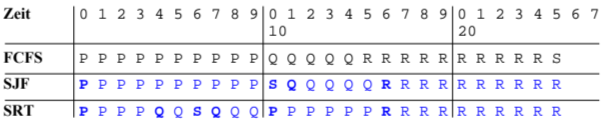
\includegraphics[width=\linewidth]{SCHEDULING_sep07.png}
\end{example2}

\begin{KR}{Scheduling Algorithm Analysis}
    \paragraph{FIFO/FCFS approach}
    \begin{itemize}
        \item Execute processes in arrival order
        \item Non-preemptive
        \item Simple but may cause long wait times
    \end{itemize}
    
    \paragraph{SJF approach}
    \begin{itemize}
        \item At decision point, choose process with shortest total time
        \item Non-preemptive
        \item Optimal for average waiting time
    \end{itemize}
    
    \paragraph{SRT approach}
    \begin{itemize}
        \item At each time unit, choose process with shortest remaining time
        \item Preemptive version of SJF
        \item May cause frequent context switches
    \end{itemize}
    
    \paragraph{Problem-solving steps}
    \begin{itemize}
        \item Create timeline showing all events (arrivals, completions)
        \item For each algorithm, trace through decision points
        \item Calculate metrics: turnaround time, waiting time, response time
    \end{itemize}
\end{KR}

\begin{example2}{Round Robin Scheduling}
    Why should the time quantum be larger than typical interaction time?
    
    \tcblower
    
    \textbf{Reason:}
    If the quantum is larger than interaction processing time, the entire user interaction can be completed within one quantum. This ensures the system responds quickly to user input without interrupting the interactive process.
    
    If the quantum is too small, interactive processes get interrupted before completing their response, leading to poor user experience.
\end{example2}

\begin{KR}{Round Robin Analysis}
    \paragraph{Quantum size considerations}
    \begin{itemize}
        \item Too large: Approaches FIFO, poor response time
        \item Too small: High context switching overhead
        \item Optimal: Slightly larger than typical interaction time
    \end{itemize}
    
    \paragraph{Performance factors}
    \begin{itemize}
        \item Context switch overhead
        \item Interactive response requirements
        \item CPU-bound vs. I/O-bound process mix
        \item System throughput vs. responsiveness trade-off
    \end{itemize}
\end{KR}

\subsection{System Calls and Memory Management}

\begin{example2}{System Call Analysis}
    Analyze the output of a program using fork() and exec():
    
\begin{lstlisting}[language=C, style=basesmol]
int pid = fork();
printf("%s\n", "[1] Time for case distinction");
if (pid) {
    printf("%s\n", "[2] Starting emacs/fstab");
    execl("/bin/emacs", "/etc/fstab", (char *)NULL);
} else {
    printf("%s\n", "[3] Starting emacs/hosts");
    execl("/bin/emacs", "/etc/hosts", (char *)NULL);
}
printf("%s\n", "[4] Two editors started successfully");
// More code follows...
\end{lstlisting}
    
    \tcblower
    
    \textbf{Analysis:}\\
    Programm startet mit 2 Editoren:\\
    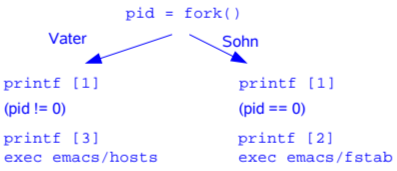
\includegraphics[width=0.5\linewidth]{system_calls_SEP07.png}

    \begin{itemize}
        \item Two editors are started
        \item Output: [1], [1], [2], [3]
        \item The code after execl() calls is never reached
        \item execl() replaces the process image, so [4] is never printed
    \end{itemize}
    
    \textbf{Execution flow:}
    \begin{itemize}
        \item fork() creates parent and child
        \item Both print [1]
        \item Parent (pid $\neq$ 0) prints [2], then execl() replaces it with emacs
        \item Child (pid == 0) prints [3], then execl() replaces it with emacs
    \end{itemize}
\end{example2}

\begin{KR}{Fork and Exec Analysis}
    \paragraph{Key concepts}
    \begin{itemize}
        \item fork() duplicates current process
        \item exec() family replaces current process image
        \item Code after exec() only runs if exec() fails
        \item Count processes by tracing fork() calls
    \end{itemize}
    
    \paragraph{Analysis steps}
    \begin{itemize}
        \item Draw execution tree showing parent/child branches
        \item Mark where each printf() executes
        \item Identify exec() calls that replace process image
        \item Determine unreachable code after successful exec()
    \end{itemize}
\end{KR}

\begin{example2}{Virtual Memory Address Translation}
    Given: 16KB page size, 47-bit virtual addresses, 3-level paging, 8-byte page table entries.
    
    How is a virtual address structured?
    
    \tcblower
    
    \textbf{Calculation:}
    \begin{itemize}
        \item Page size: 16KB = 2\textsuperscript{14} bytes $\rightarrow$ 14 bits for page offset
        \item Remaining bits: 47 - 14 = 33 bits for page table indexing
        \item 3 levels: 33 ÷ 3 = 11 bits per page table level
    \end{itemize}
    
    \textbf{Address structure:}
    \begin{tabular}{|c|c|c|c|}
        \hline
        Bits 46-36 & Bits 35-25 & Bits 24-14 & Bits 13-0 \\
        \hline
        Level 1 (11 bit) & Level 2 (11 bit) & Level 3 (11 bit) & Offset (14 bit) \\
        \hline
    \end{tabular}
    
    \textbf{Page table sizes:}
    \begin{itemize}
        \item Level 1: 1 table with 2\textsuperscript{11} = 2048 entries
        \item Level 2: 2048 tables with 2048 entries each
        \item Level 3: 2048\textsuperscript{2} = 4,194,304 tables with 2048 entries each
        \item Each table: 2048 × 8 bytes = 16KB (exactly one page)
    \end{itemize}
\end{example2}

\begin{KR}{Virtual Memory Address Analysis}
    \paragraph{Address structure calculation}
    \begin{itemize}
        \item Page offset bits = $log_2$(page size in bytes)
        \item Remaining bits = total address bits - offset bits
        \item Bits per level = remaining bits ÷ number of levels
    \end{itemize}
    
    \paragraph{Page table size calculation}
    \begin{itemize}
        \item Entries per table = 2\textsuperscript{bits per level}
        \item Table size = entries × entry size in bytes
        \item Number of tables per level = cumulative from higher levels
    \end{itemize}
    
    \paragraph{Common mistakes to avoid}
    \begin{itemize}
        \item Forgetting to account for page offset bits
        \item Mixing up table levels in size calculations
        \item Not considering that tables should fit in pages
    \end{itemize}
\end{KR}

\important{ADD EXERCISE 12 SEP07 SEGMENTATION}

\raggedcolumns
\columnbreak

\subsection{Synchronization and File Systems}

\begin{example2}{Producer-Consumer Problem}
    Implement a semaphore-based solution for the producer-consumer problem:
    
    \tcblower
    
\begin{lstlisting}[language=C, style=basesmol]
const int N = 4;        // Maximum buffer size
int sem_write = N;      // Semaphore for write slots
int sem_read = 0;       // Semaphore for read slots

// Producer process
while(1) {
    wait(sem_write);    // Wait for empty slot
    write(value);       // Write to buffer
    signal(sem_read);   // Signal data available
}

// Consumer process  
while(1) {
    wait(sem_read);     // Wait for data
    read(value);        // Read from buffer
    signal(sem_write);  // Signal slot available
}
\end{lstlisting}

    \textbf{Key points:}
    \begin{itemize}
        \item sem\_write tracks empty buffer slots
        \item sem\_read tracks filled buffer slots
        \item Producer waits for empty slots, signals filled slots
        \item Consumer waits for filled slots, signals empty slots
    \end{itemize}
\end{example2}

\begin{KR}{Synchronization Problem Solving}
    \paragraph{Producer-Consumer pattern}
    \begin{itemize}
        \item Identify shared resource (buffer)
        \item Determine capacity constraints
        \item Create semaphores for available/used slots
        \item Producer: wait(empty), produce, signal(full)
        \item Consumer: wait(full), consume, signal(empty)
    \end{itemize}
    
    \paragraph{General synchronization approach}
    \begin{itemize}
        \item Identify critical sections
        \item Determine synchronization requirements
        \item Choose appropriate mechanism (mutex, semaphore, monitor)
        \item Ensure deadlock avoidance
        \item Test for race conditions
    \end{itemize}
\end{KR}

\begin{example2}{File System Free Space Management}
    Describe two efficient methods for tracking free blocks:
    
    \tcblower
    
    \textbf{Method 1: Bitmap}
    \begin{itemize}
        \item Each bit represents one block
        \item 0 = free, 1 = allocated (or vice versa)
        \item Fast scanning for free blocks
        \item Compact representation
        \item Requires main memory for efficiency
    \end{itemize}
    
    \textbf{Method 2: Free block list with (start, length) tuples}
    \begin{itemize}
        \item List of contiguous free block ranges
        \item Each entry: (starting block, number of blocks)
        \item Efficient for large contiguous areas
        \item Dynamic size based on fragmentation
    \end{itemize}
\end{example2}

\begin{KR}{File System Design Analysis}
    \paragraph{Free space management methods}
    \begin{itemize}
        \item Bitmap: Good for uniform access, fixed size
        \item Linked list: Simple but slow random access
        \item Grouping: Combines free blocks into groups
        \item Counting: Stores (address, count) pairs
    \end{itemize}
    
    \paragraph{Evaluation criteria}
    \begin{itemize}
        \item Space efficiency
        \item Access speed
        \item Implementation complexity
        \item Fragmentation handling
        \item Main memory requirements
    \end{itemize}
\end{KR}

\subsection{Page Replacement and Memory Management}

\begin{example2}{Page Replacement Algorithms}
    Compare LRU and FIFO page replacement algorithms:
    
    \tcblower
    
    \textbf{LRU (Least Recently Used) typically causes fewer page faults because:}
    \begin{itemize}
        \item Exploits locality principle
        \item Recently accessed pages likely to be accessed again soon
        \item Keeps "hot" pages in memory longer
        \item Better prediction of future access patterns
    \end{itemize}
    
    \textbf{FIFO (First In, First Out):}
    \begin{itemize}
        \item Simple implementation
        \item No consideration of access patterns
        \item May replace frequently used pages
        \item Can suffer from Belady's anomaly
    \end{itemize}
    
    \textbf{Optimal algorithm (theoretical):}
    \begin{itemize}
        \item Replace page that will be accessed furthest in future
        \item Not implementable (requires future knowledge)
        \item Used as performance benchmark
    \end{itemize}
\end{example2}

\begin{KR}{Page Replacement Analysis}
    \paragraph{Algorithm comparison factors}
    \begin{itemize}
        \item Page fault frequency
        \item Implementation complexity
        \item Hardware support requirements
        \item Performance under different workloads
        \item Memory overhead for bookkeeping
    \end{itemize}
    
    \paragraph{Common algorithms}
    \begin{itemize}
        \item FIFO: Simple, poor performance
        \item LRU: Good performance, moderate complexity
        \item Clock: Approximates LRU, hardware efficient
        \item Optimal: Theoretical best, not implementable
    \end{itemize}
\end{KR}

\raggedcolumns
\columnbreak

\subsection{Advanced Topics}

\begin{example2}{Priority Inversion Problem}
    Explain priority inversion and how to prevent it:
    
    \tcblower
    
    \textbf{Priority inversion occurs when:}
    \begin{itemize}
        \item High-priority process waits for low-priority process
        \item Medium-priority processes preempt low-priority process
        \item High-priority process effectively blocked by medium-priority processes
    \end{itemize}
    
    \textbf{Prevention methods:}
    \begin{itemize}
        \item \textbf{Priority inheritance}: Low-priority process temporarily inherits high priority
        \item \textbf{Priority ceiling}: Resources assigned maximum priority of potential users
        \item \textbf{Dynamic priority adjustment}: Increase priority of waiting processes over time
    \end{itemize}
\end{example2}

\begin{KR}{Priority-Based Scheduling Issues}
    \paragraph{Common priority problems}
    \begin{itemize}
        \item Priority inversion
        \item Starvation of low-priority processes
        \item Priority assignment difficulties
        \item Real-time deadline misses
    \end{itemize}
    
    \paragraph{Solution approaches}
    \begin{itemize}
        \item Priority inheritance protocols
        \item Aging mechanisms
        \item Fair-share scheduling
        \item Deadline-based scheduling
    \end{itemize}
\end{KR}

\begin{example2}{Linux O(1) Scheduler}
    Explain why the Linux O(1) scheduler is called O(1):
    
    \tcblower
    
    \textbf{O(1) refers to constant time complexity:}
    \begin{itemize}
        \item Time to find next process is independent of total number of processes
        \item Uses active and expired arrays with 140 priority levels each
        \item Bitmap indicates which priority levels have waiting processes
        \item Simply finds highest priority bit set and takes first process from that queue
    \end{itemize}
    
    \textbf{Algorithm:}
    \begin{itemize}
        \item Check bitmap for highest priority with waiting processes
        \item Take first process from that priority queue
        \item Constant time regardless of system load
    \end{itemize}
\end{example2}

\begin{KR}{Algorithm Complexity Analysis}
    \paragraph{Time complexity evaluation}
    \begin{itemize}
        \item O(1): Constant time, independent of input size
        \item O(log n): Logarithmic time, scales well
        \item O(n): Linear time, proportional to input size
        \item Identify bottleneck operations
    \end{itemize}
    
    \paragraph{Scheduler efficiency factors}
    \begin{itemize}
        \item Process selection time
        \item Context switch overhead
        \item Load balancing cost
        \item Priority calculation complexity
    \end{itemize}
\end{KR}